\section{Эксперименты} \label{experiments}

\subsection{Методика и тестовое окружение}

Все эксперименты, требовавшие точных измерений времени, выполнялись с помощью фреймворка Google Benchmark; число повторений подбиралось автоматически для получения стабильных результатов. Измерения проводились на стенде со следующими характеристиками:

\begin{itemize}
    \item Центральный процессор: AMD Ryzen 5 5600 (6 ядер / 12 потоков), максимальная частота до 4,47 ГГц, кэш L3 32 МБ.
    \item Оперативная память: 32 ГБ DDR4-2666 (Kingston, 2×16 ГБ).
    \item Накопитель: SSD Kingston SNV3S1000G (NVMe, 1 ТБ).
    \item Материнская плата: Gigabyte B550M DS3H R2.
    \item Операционная система: Ubuntu 24.04.3 LTS, ядро 6.17.0-23-generic.
\end{itemize}

В качестве тестовых данных использовался файл \texttt{webster} из корпуса сжатия Силезского университета (Silesia compression corpus). Этот файл содержит несжатый текст The 1913 Webster Unabridged Dictionary, сохранённый в HTML-разметке; размер составляет примерно 40 МБ, но он был обрезан до 32 МБ.

Там, где требовалось изолировать эффект от кэширования, кэш блоков и/или узлов принудительно очищался вызовом \texttt{compio\_flush} после каждой операции. В остальных случаях параметры кэшей определялись настройками по умолчанию и отдельно оговариваются.

\subsection{Борьба с внутренней фрагментацией}

\paragraph{Постановка эксперимента.}
Для проверки эффективности стратегии управления размерами блоков с помощью границ \texttt{block\_size\_minimum} и \texttt{block\_size\_maximum} моделировался длительный поток случайных вставок и удалений внутри логического файла размером 32 МБ. Сравнивались два варианта:

\begin{itemize}
    \item \textbf{Наивный} --- блоки не сливаются и не перераспределяются целенаправленно. При вставке в середину блока он разрезается на два; при вставке между блоками создаётся новый блок с размером, равным вставляемым данным; при удалении крайние затронутые блоки делятся, а внутренние удаляются; дополнение файла записывается блоками целевого размера \texttt{block\_size}. Без механизма слияния размеры блоков неограниченно уменьшаются.
    \item \textbf{С диапазоном} --- используются пороги \texttt{block\_size\_minimum} и \texttt{block\_size\_maximum}: слишком маленькие блоки сливаются с соседними, слишком большие разделяются на несколько блоков.
\end{itemize}

В ходе эксперимента измерялись количество блоков в B-дереве и средняя скорость операций (МБ/с) после каждого шага.

\paragraph{Результаты.}
На рис.~\ref{fig:fragmentation} видно, что без регулировки число блоков монотонно растёт и после нескольких тысяч операций достигает десятков тысяч. Это приводит к углублению B-дерева, росту числа дисковых операций и падению скорости до 2--3 МБ/с. При использовании диапазона размеров количество блоков стабилизируется на уровне 300--400, а скорость сохраняется в пределах 20--30 МБ/с (небольшое снижение связано с другими факторами, такими как внешняя фрагментация).

\begin{figure}[h]
    \centering
    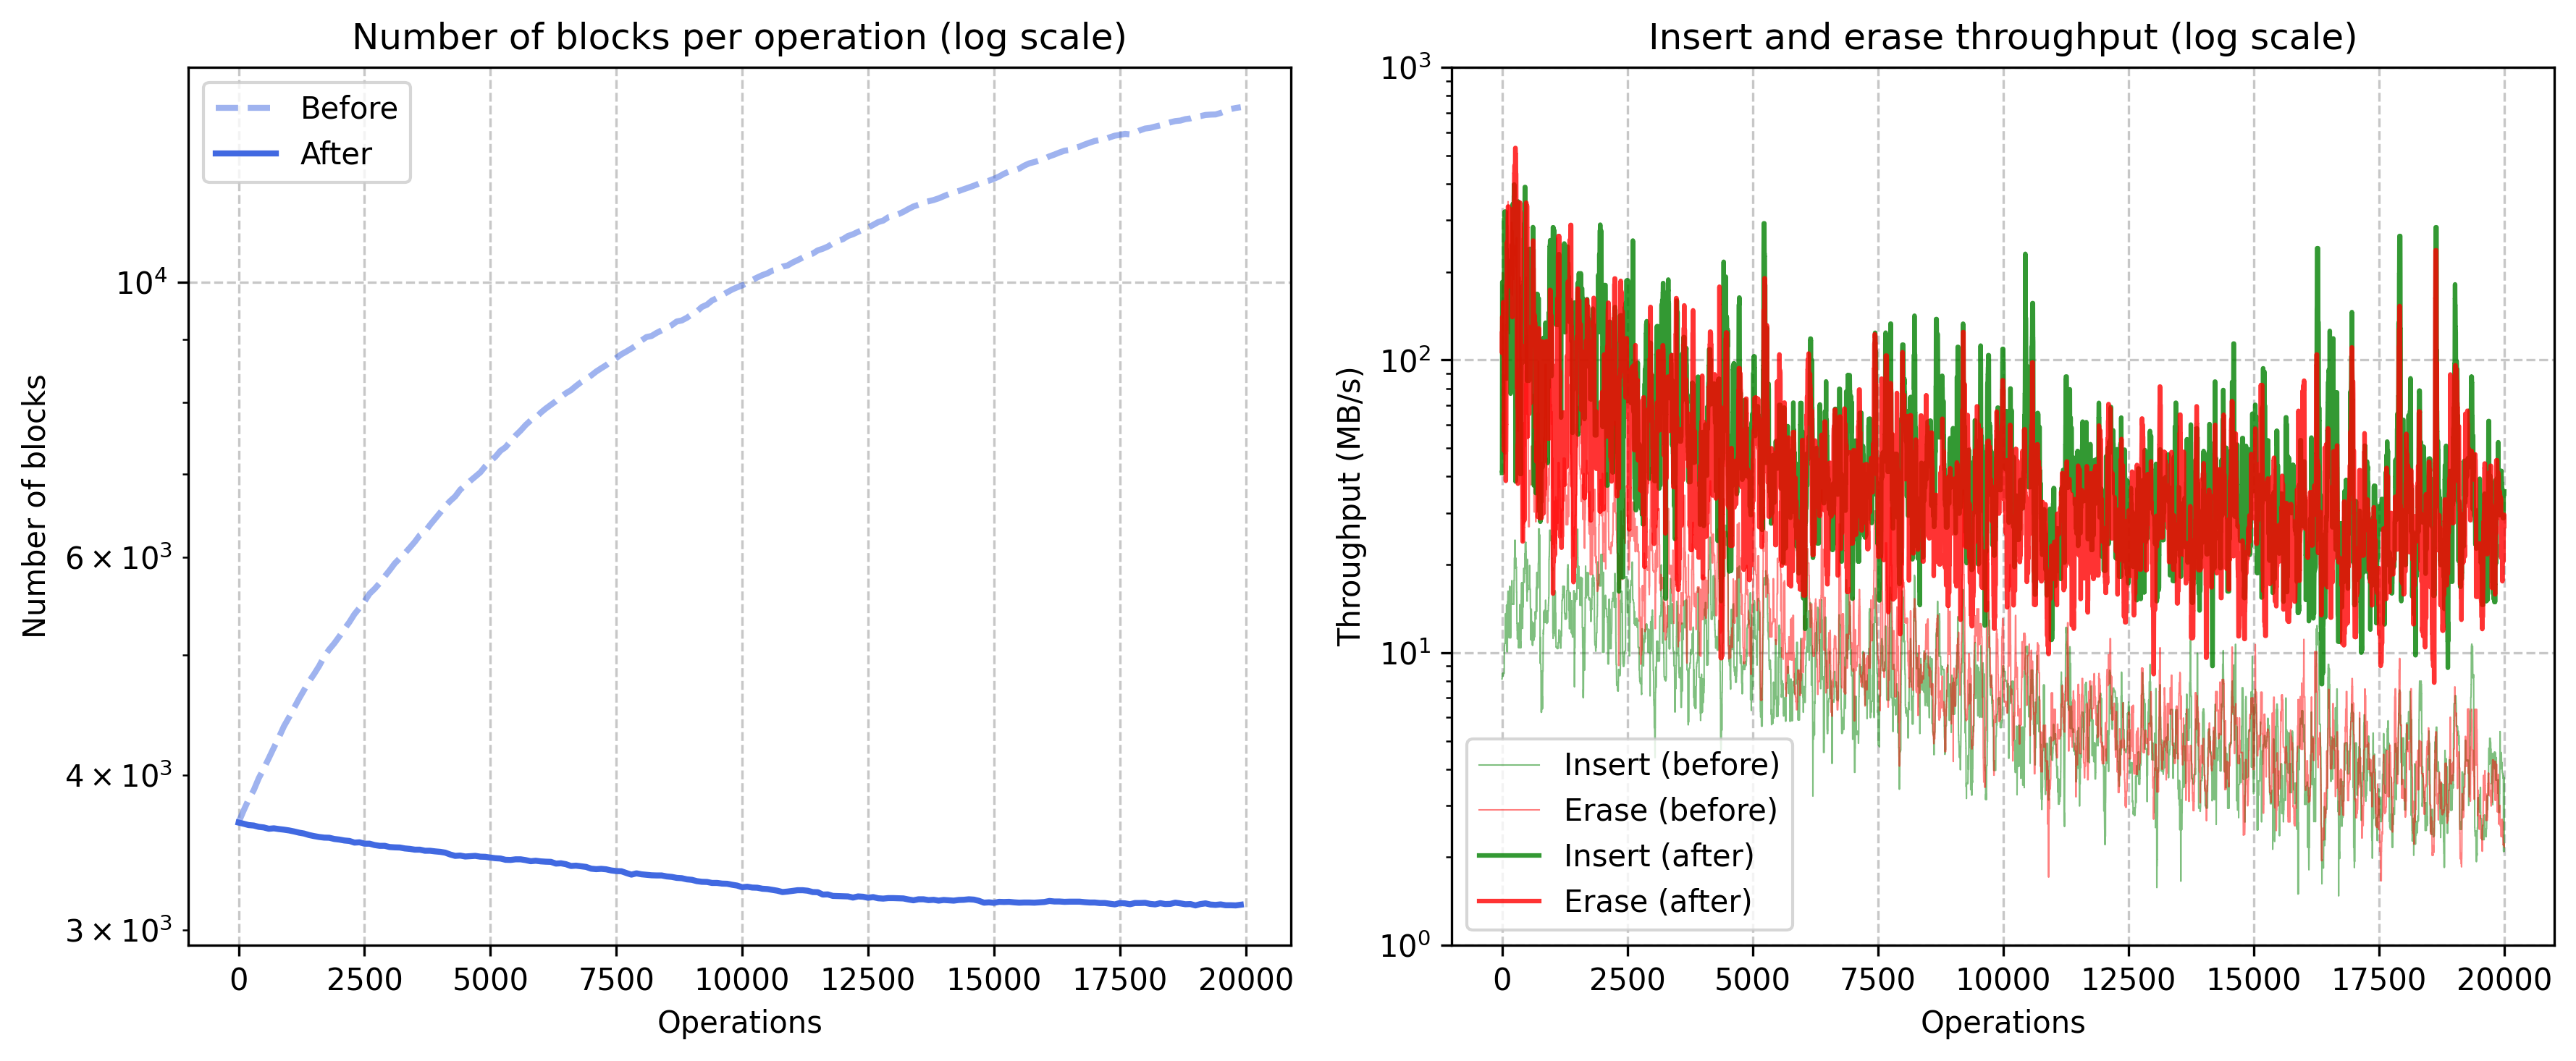
\includegraphics[width=\textwidth]{images/internal_fragmentation.png}
    \caption{Влияние стратегии управления логическими блоками на количество блоков и скорость вставки/удаления.}
    \label{fig:fragmentation}
\end{figure}

\paragraph{Вывод.}
Механизм \texttt{block\_size\_minimum} и \texttt{block\_size\_maximum} надёжно предотвращает деградацию производительности, вызванную внутренней фрагментацией, и оправдывает проектное решение, заложенное в архитектуру библиотеки.

\subsection{Произвольное чтение: сравнение с аналогами}

\paragraph{Краткое описание инструментов.}
\textit{Seekable zstd} разбивает входные данные на независимые кадры (frames), каждый из которых сжимается алгоритмом Zstd с полным сбросом состояния. Индекс смещений кадров хранится в виде массива, поиск выполняется бинарным поиском. \textit{Zran} --- надстройка над Deflate, использующая точки останова со снимками состояния декомпрессора; при чтении распаковка начинается с ближайшей предыдущей точки, что делает метод более эффективным для крупных запросов. Оба инструмента ориентированы только на произвольное чтение; любое изменение данных требует полной распаковки и повторной упаковки всего архива.

\paragraph{Методика.}
Архив размером 32 МБ (HTML) подготавливался каждым из инструментов. Затем выполнялось 1000 случайных чтений блоков по 4 КБ в случайных позициях. У Compio кэш блоков принудительно очищался после каждой операции, чтобы условия были максимально близки к аналогам, не имеющим кэширования. Compio тестировался с компрессорами Zlib (уровень 1) и Zstd (уровень 1) --- те же алгоритмы и уровни, что использовались в seekable zstd и zran соответственно. Варьировался параметр, управляющий гранулярностью: \texttt{block\_size} у Compio, \texttt{max\_frame\_size} у seekable zstd и \texttt{flush\_interval} у zran.

\paragraph{Результаты.}
На рис.~\ref{fig:alternatives} представлен trade-off «скорость – размер архива» (логарифмические шкалы). Каждая точка соответствует одному значению параметра гранулярности.

\begin{figure}[h]
    \centering
    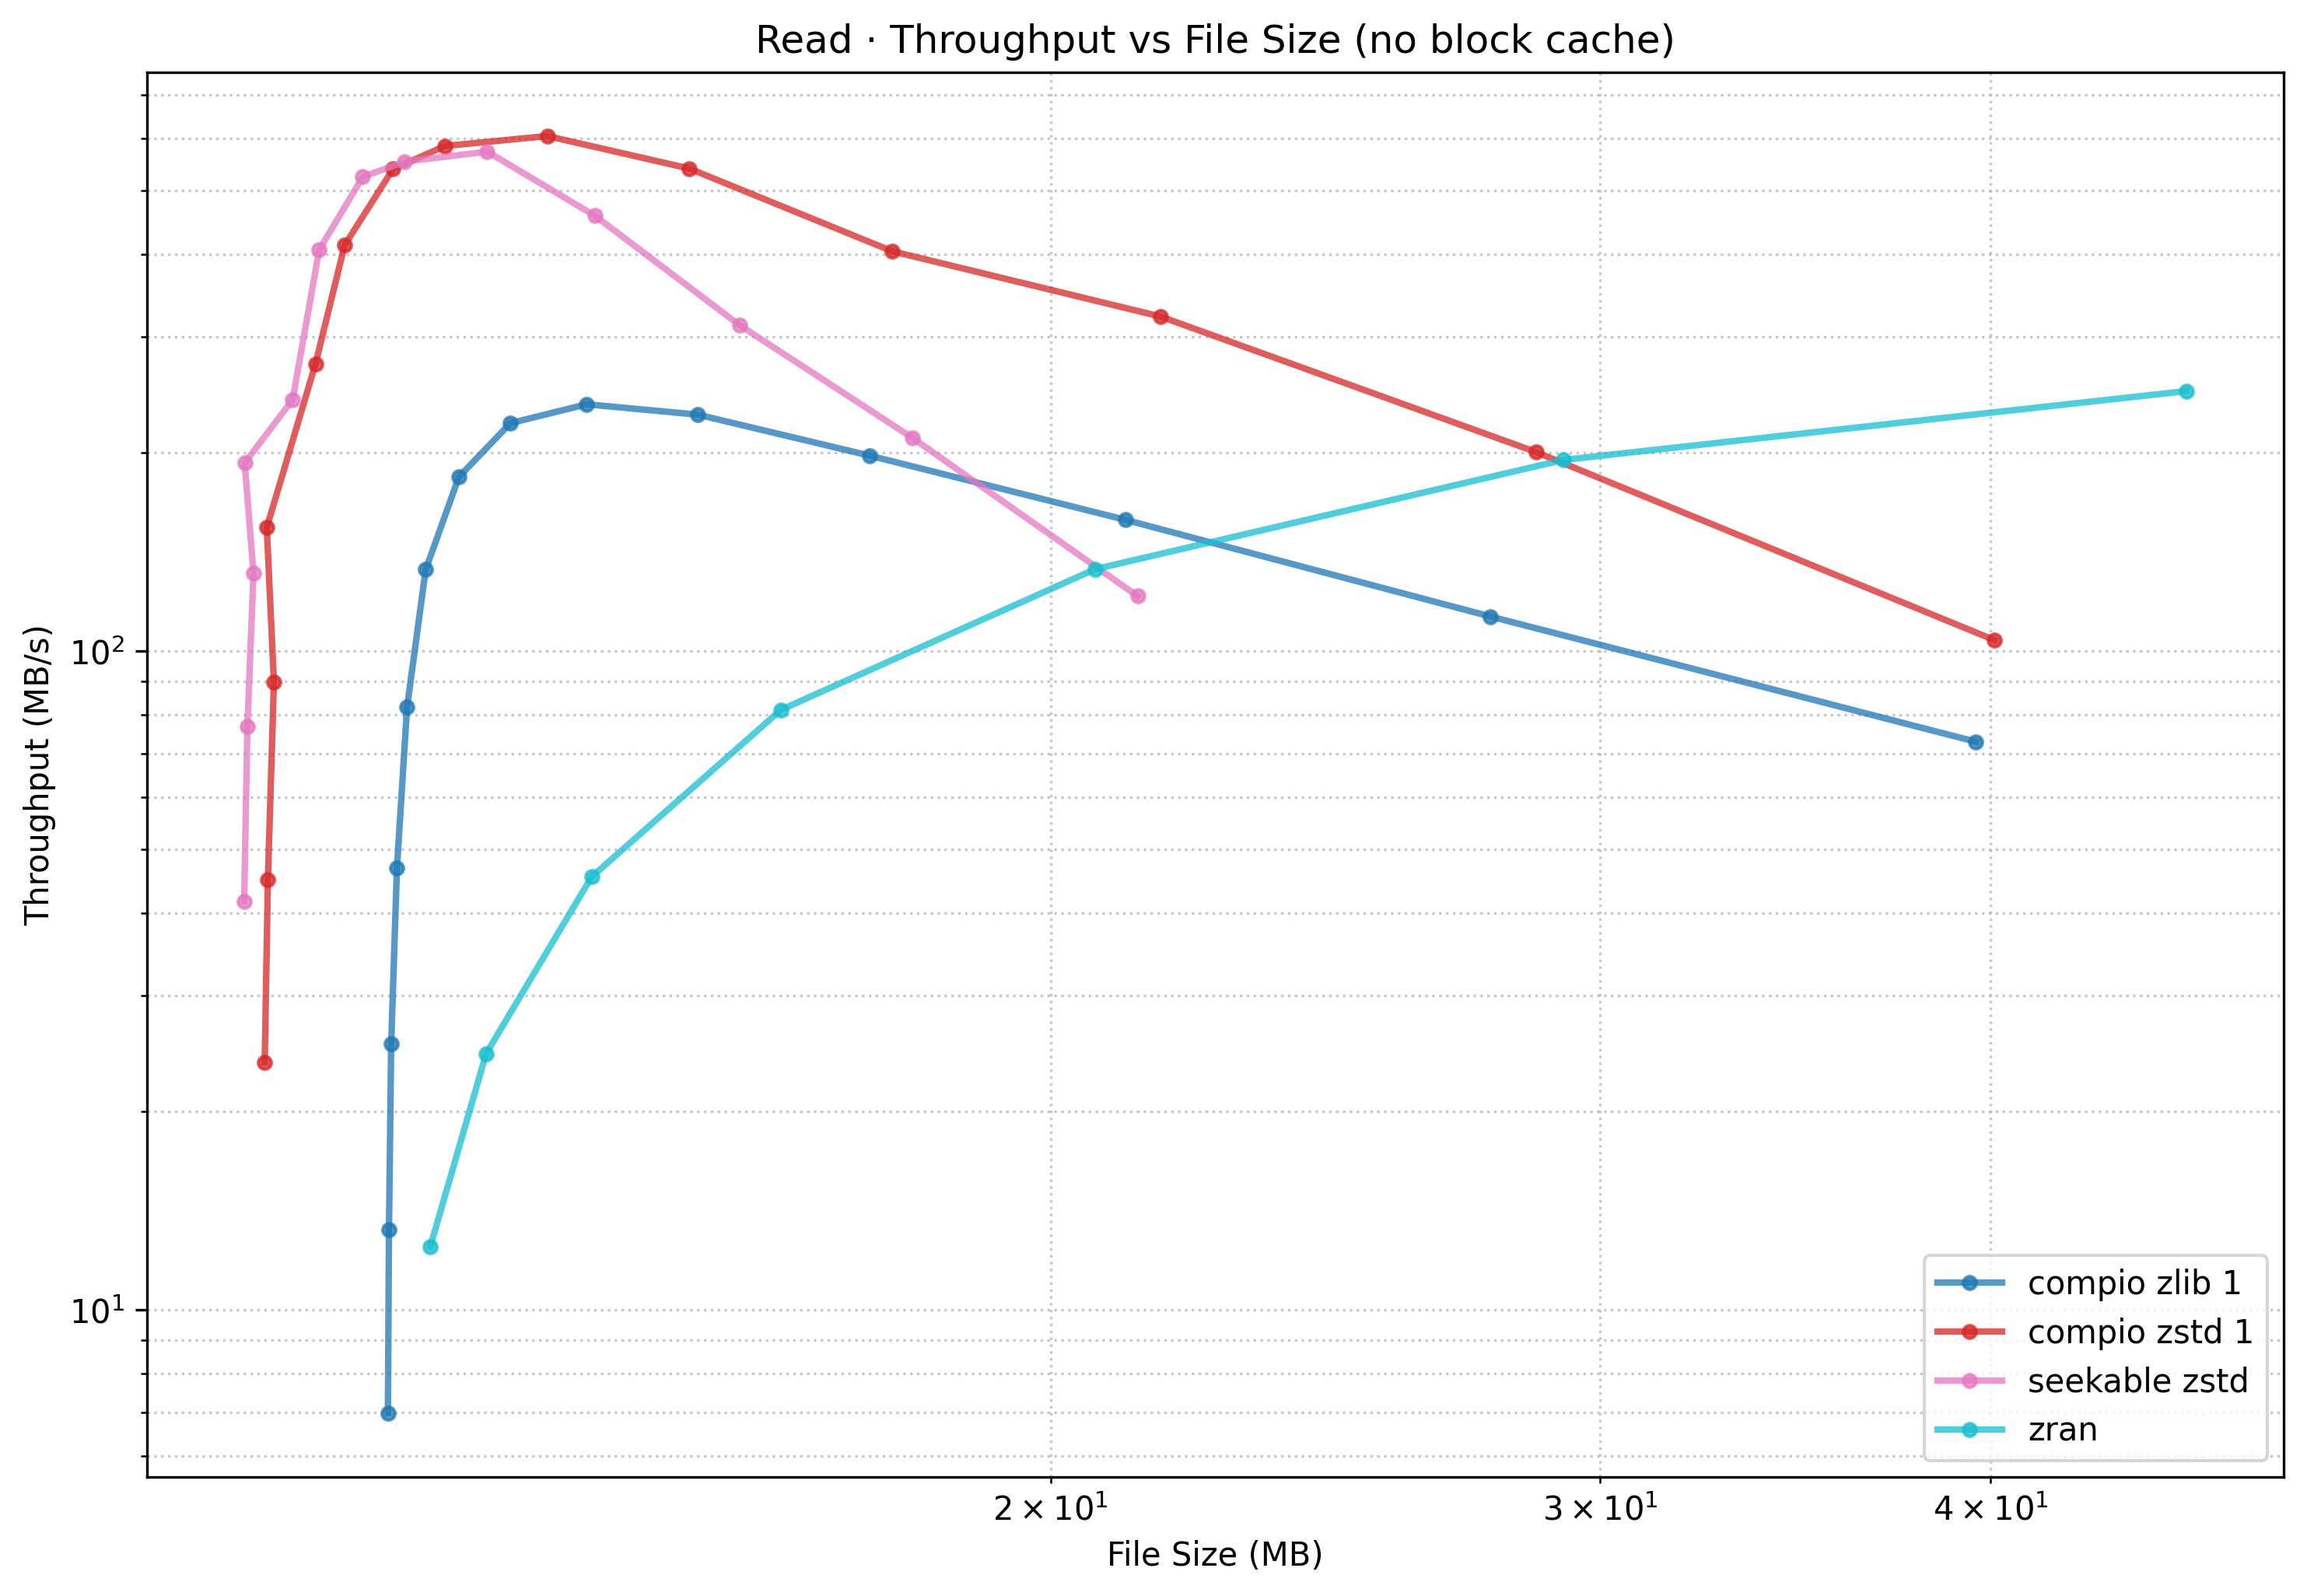
\includegraphics[width=\textwidth]{images/alternatives.png}
    \caption{Сравнение произвольного чтения: Compio (Zlib, Zstd), seekable zstd и zran.}
    \label{fig:alternatives}
\end{figure}

Для размеров блока 4--16 КБ точки Compio+Zstd и seekable zstd практически совпадают. При больших блоках (64--256 КБ) seekable zstd показывает чуть худшую скорость, однако эти режимы не являются оптимальными для произвольного доступа. Zran заметно уступает Compio+Zlib: скорость ниже, а размер файла растёт быстрее из-за большого индекса. Причина --- Zran рассчитан на чтения, сопоставимые по размеру с интервалом между точками останова, а наши запросы по 4 КБ слишком мелкие.

\paragraph{Вывод.}
Даже при отключённом кэшировании Compio не уступает специализированным инструментам в сценарии произвольного чтения, при этом оставаясь единственным решением, которое дополнительно поддерживает полноценную запись, вставку и удаление данных без перепаковки всего архива.

\subsection{Влияние кэширования и сравнение с stdio}

\paragraph{Постановка.}
Данный эксперимент демонстрирует роль кэша распакованных блоков при высокой локальности обращений и позволяет сравнить скорость работы со стандартным несжатым вводом-выводом (\texttt{stdio} с буферизацией).

Для логического файла в 32 МБ имитировалась последовательность чтений или записей с заданным процентом попаданий в кэш блоков (cache hit ratio). Этот процент регулировался вероятностью повторного обращения к уже недавно прочитанному блоку. Измерялась средняя скорость (МБ/с). Compio тестировался с компрессорами LZ4, Zstd (уровни 1 и 5), Zlib и Brotli; настройки кэша блоков использовались стандартные, без искусственного ограничения ёмкости.

Для фиксированного процента попаданий 97,5\% строился дополнительный trade-off «скорость – размер файла», чтобы учесть и степень сжатия.

\paragraph{Результаты.}
На рис.~\ref{fig:cache_read} показана скорость чтения, на рис.~\ref{fig:cache_write}~--- скорость записи. Каждый рисунок содержит две панели: левая~--- зависимость скорости от процента попаданий в кэш, правая~--- trade-off «скорость – размер» при 97,5\% попаданий.

\begin{figure}[h]
\centering
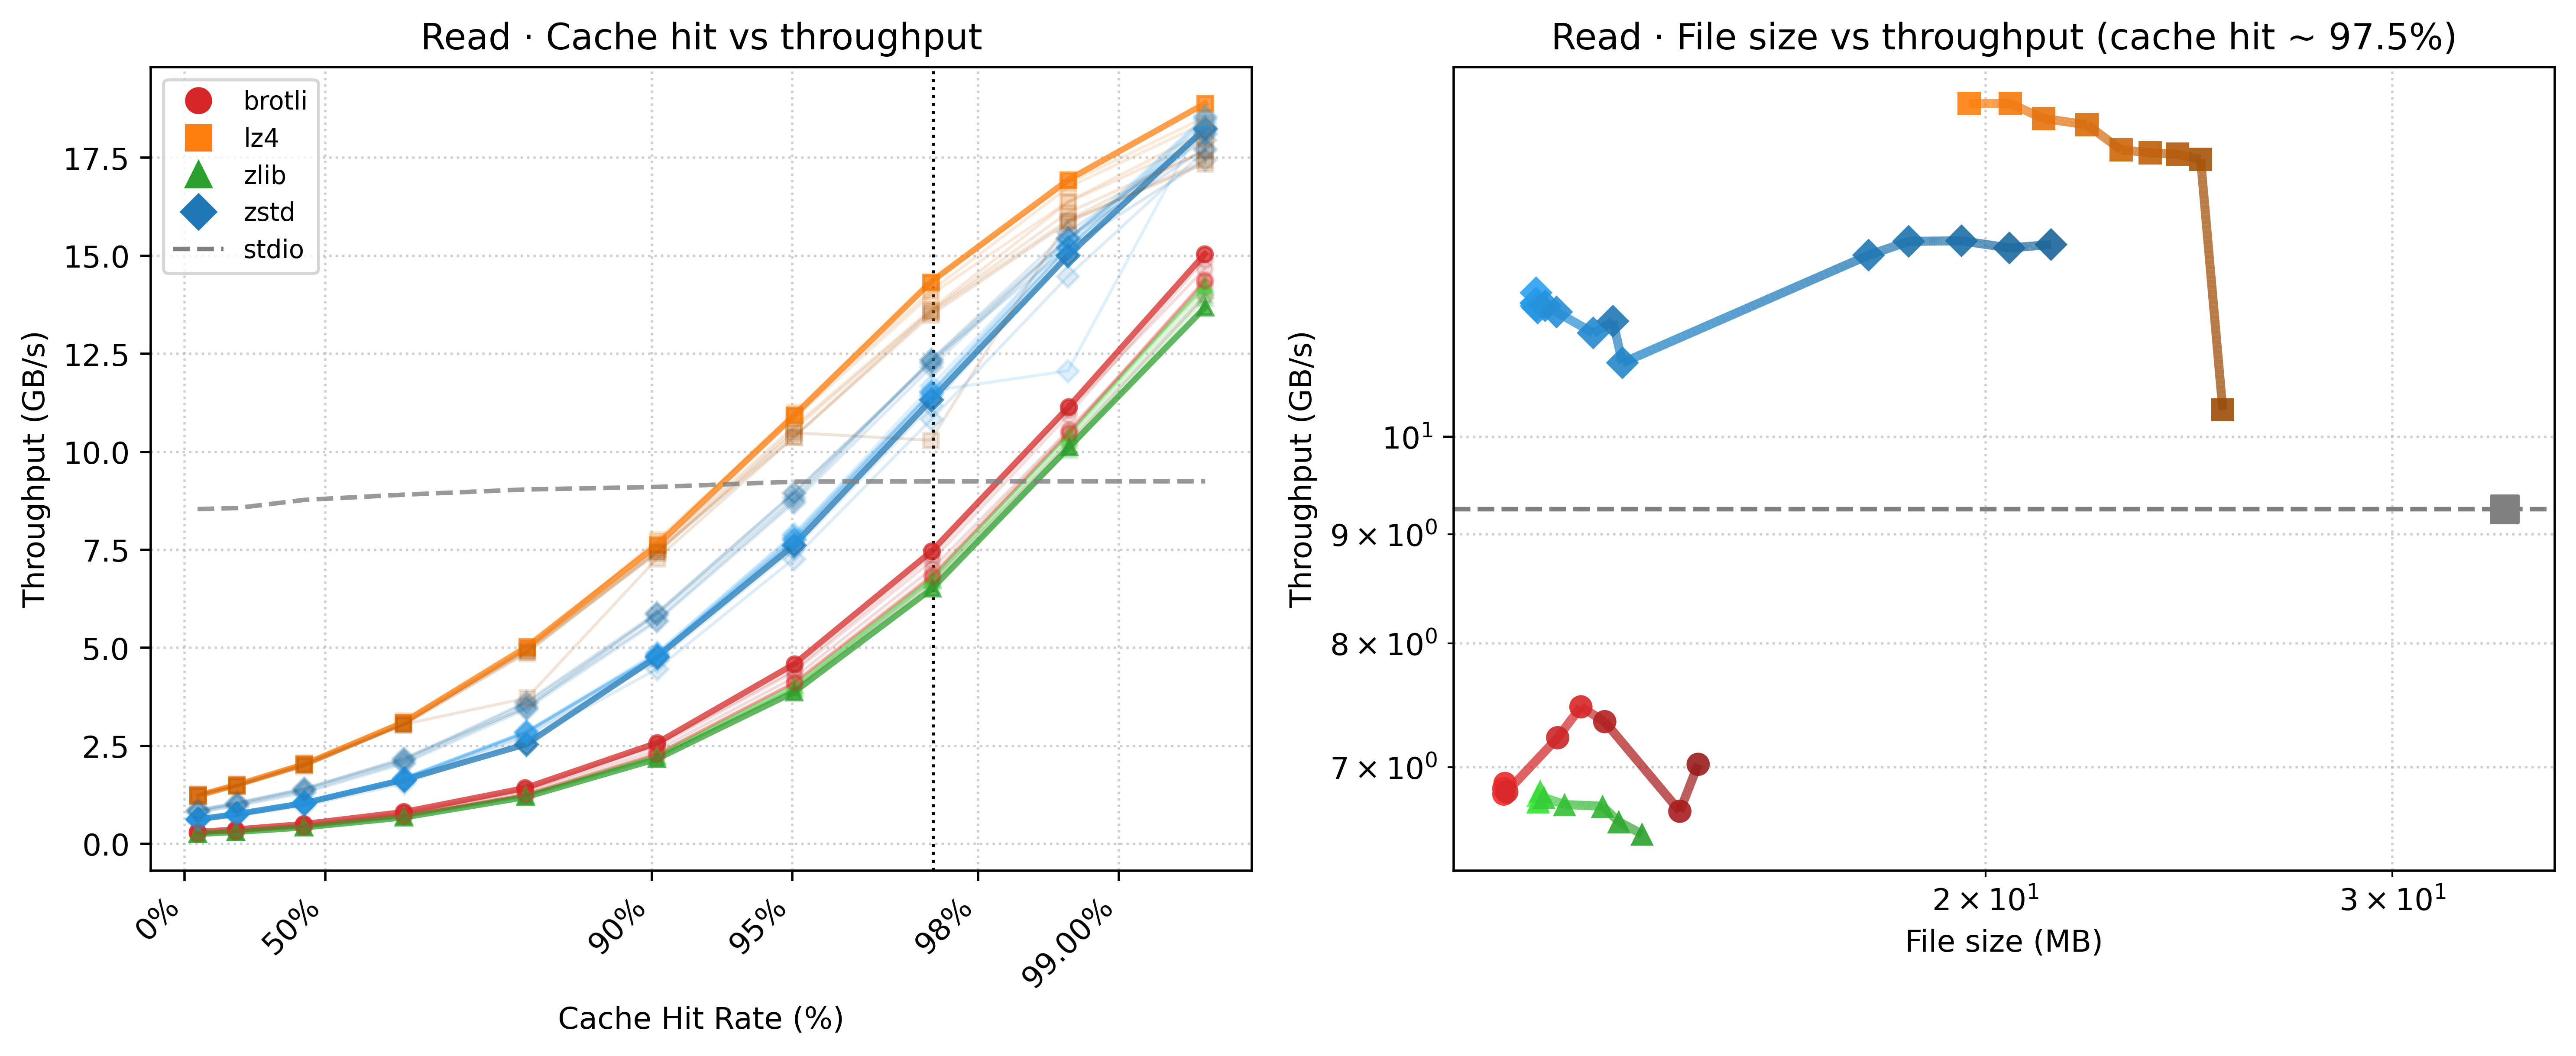
\includegraphics[width=\textwidth]{images/cache_impact_read.png}
\caption{Скорость чтения в зависимости от процента попаданий в кэш блоков (слева) и trade-off «скорость – размер файла» при фиксированной локальности 97,5\% (справа).}
\label{fig:cache_read}
\end{figure}

\begin{figure}[h]
\centering
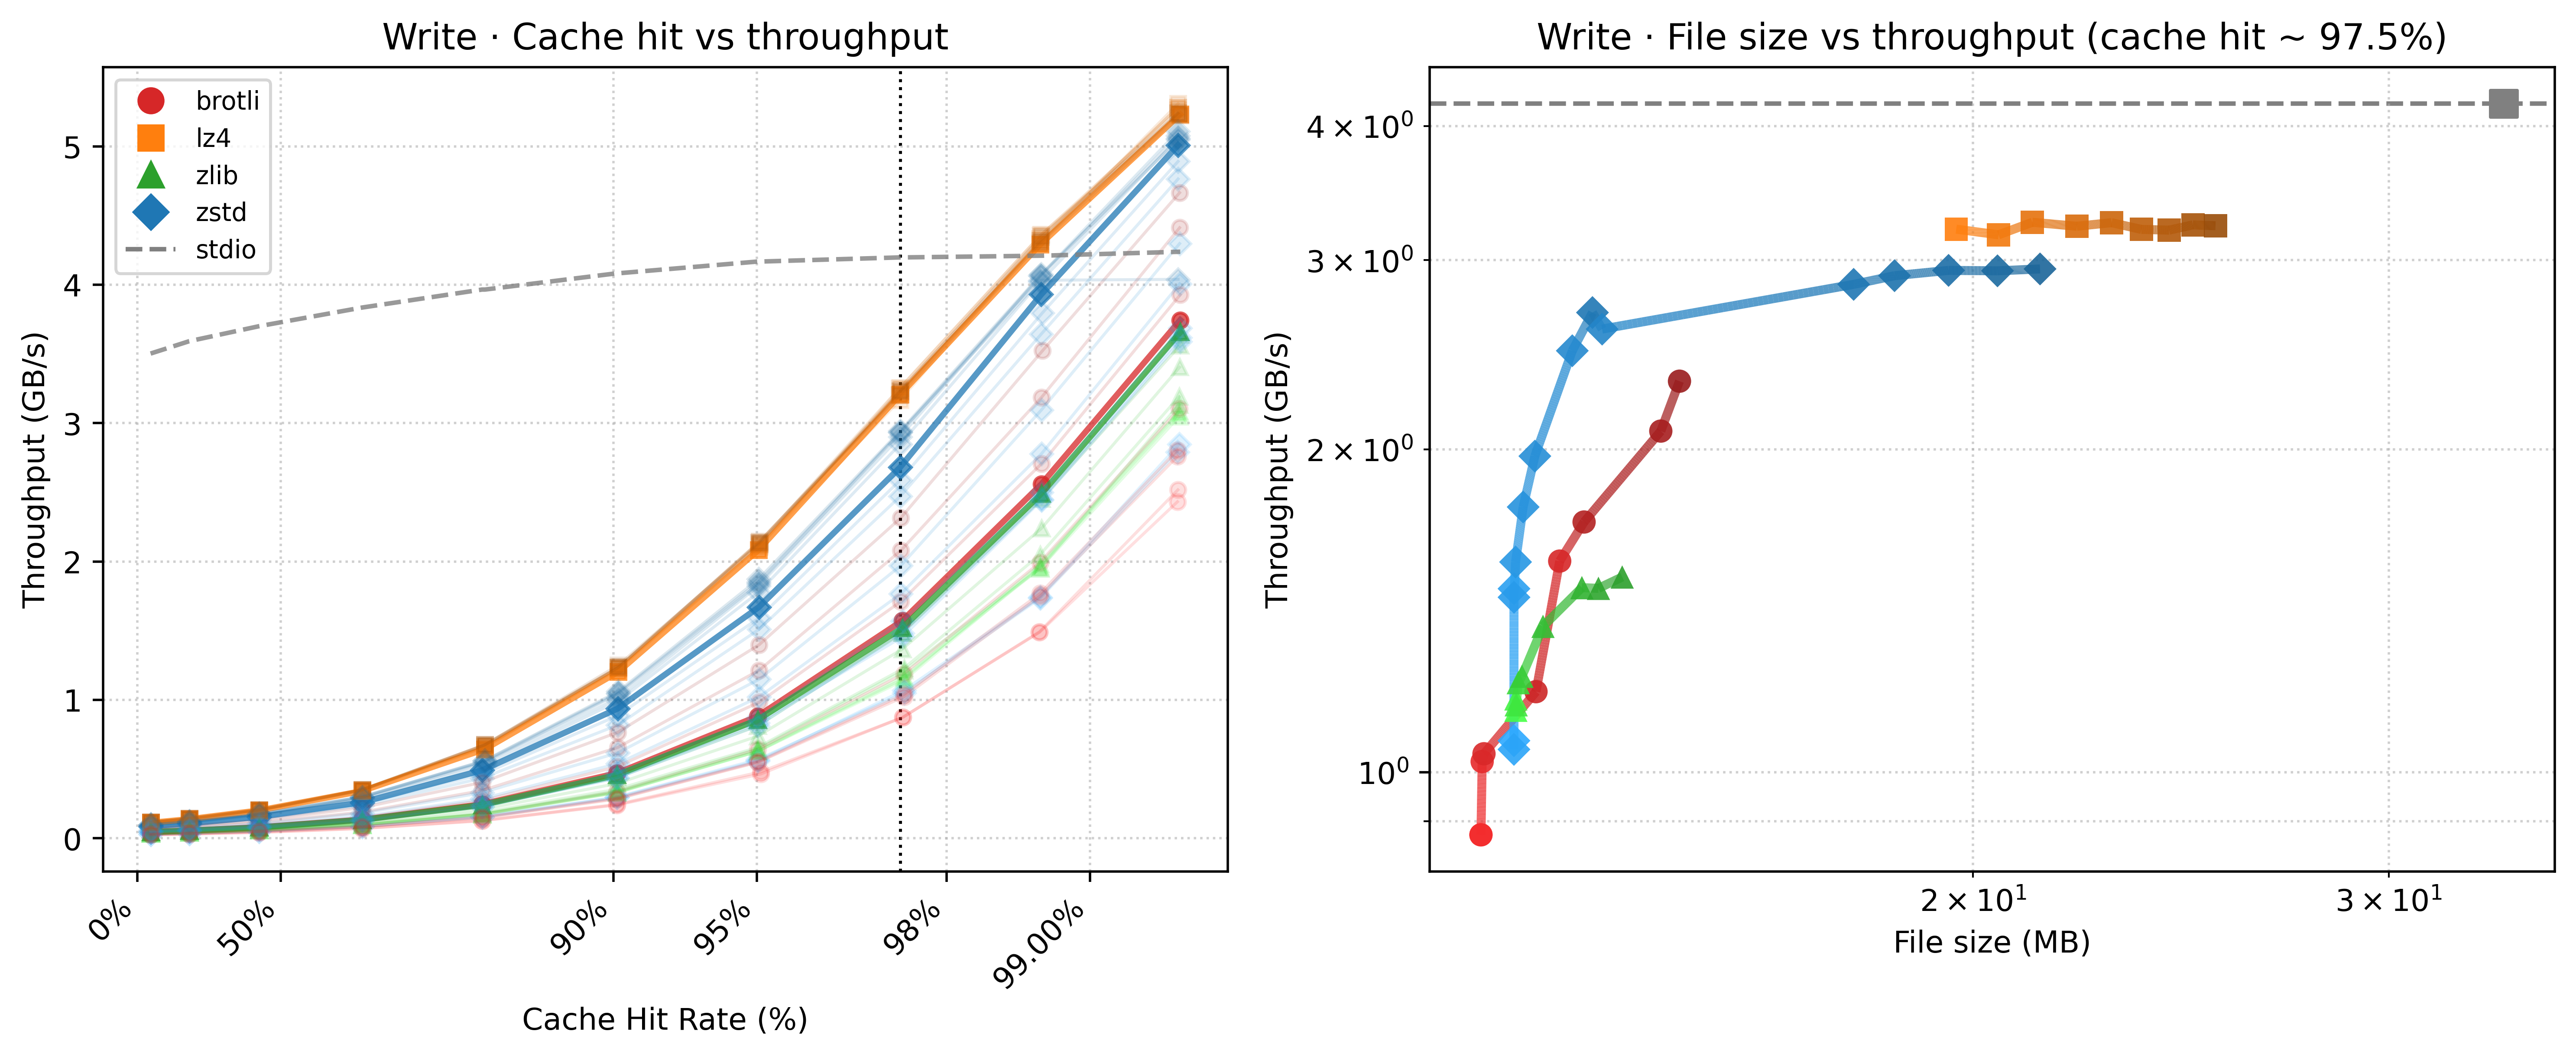
\includegraphics[width=\textwidth]{images/cache_impact_write.png}
\caption{Скорость записи в зависимости от процента попаданий в кэш блоков (слева) и trade-off «скорость – размер файла» при фиксированной локальности 97,5\% (справа).}
\label{fig:cache_write}
\end{figure}

При нулевой локальности Compio ожидаемо медленнее stdio из-за накладных расходов на декомпрессию/компрессию и навигацию по B-дереву. С ростом попаданий скорость быстро увеличивается. Для чтения (рис.~\ref{fig:cache_read}, слева) при >90\% попаданий многие компрессоры (особенно LZ4 и Zstd) превосходят stdio: данные уже распакованы и находятся в оперативной памяти, операция сводится к копированию в буфер пользователя. Для записи (рис.~\ref{fig:cache_write}, слева) порог превосходства выше~--- >99\%; при 90--99\% скорость сравнима со stdio, но остаётся в 2--5 раз ниже, поскольку периодически требуется сжатие и синхронизация изменённых блоков с диском.

Правые панели на обоих рисунках подтверждают, что наивысшую скорость даёт LZ4, однако ценой большого объёма файла. Zstd с уровнем сжатия 1 обеспечивает наилучший баланс: скорость близка к LZ4, а размер значительно меньше. Zlib и Brotli при высоких уровнях дают сильное сжатие, но заметно медленнее.

\paragraph{Вывод.}
Кэш блоков превращает Compio из решения, уступающего stdio на случайных запросах, в систему, способную при высокой локальности превзойти несжатый ввод-вывод (на чтение) и вплотную приблизиться к нему на запись, одновременно экономя дисковое пространство. Выбор компрессора позволяет гибко регулировать компромисс между скоростью и размером.

\subsection{Влияние размера блока на скорость и сжатие: сравнение алгоритмов}

\paragraph{Мотивация.}
Размер блока \texttt{block\_size} напрямую влияет как на скорость операций, так и на итоговый размер архива. Цель эксперимента --- исследовать совместное влияние размера блока и выбора алгоритма сжатия на производительность произвольной записи и степень сжатия, а также определить конфигурацию, обеспечивающую наилучший баланс.

\paragraph{Методика.}
На тестовом HTML-файле (32 МБ) выполнялось 1000 случайных операций записи блоками по 4 КБ в случайные позиции. Эксперимент повторялся для разных значений \texttt{block\_size} (от 1 КБ до 256 КБ) и для нескольких компрессоров: LZ4, Zstd, Zlib и Brotli. Для каждого алгоритма варьировался уровень сжатия (соответствующие точки на графике показаны разными оттенками одного цвета). Чтобы изолировать эффект от кэширования, после каждой операции принудительно вызывался \texttt{compio\_flush}, очищающий кэш блоков и узлов.

\paragraph{Результаты.}
На рис.~\ref{fig:algorithms_no_cache} каждая линия соединяет точки одного компрессора при разных размерах блока; направление вдоль линии соответствует уменьшению \texttt{block\_size} (от больших блоков слева к малым справа).

\begin{figure}[h]
    \centering
    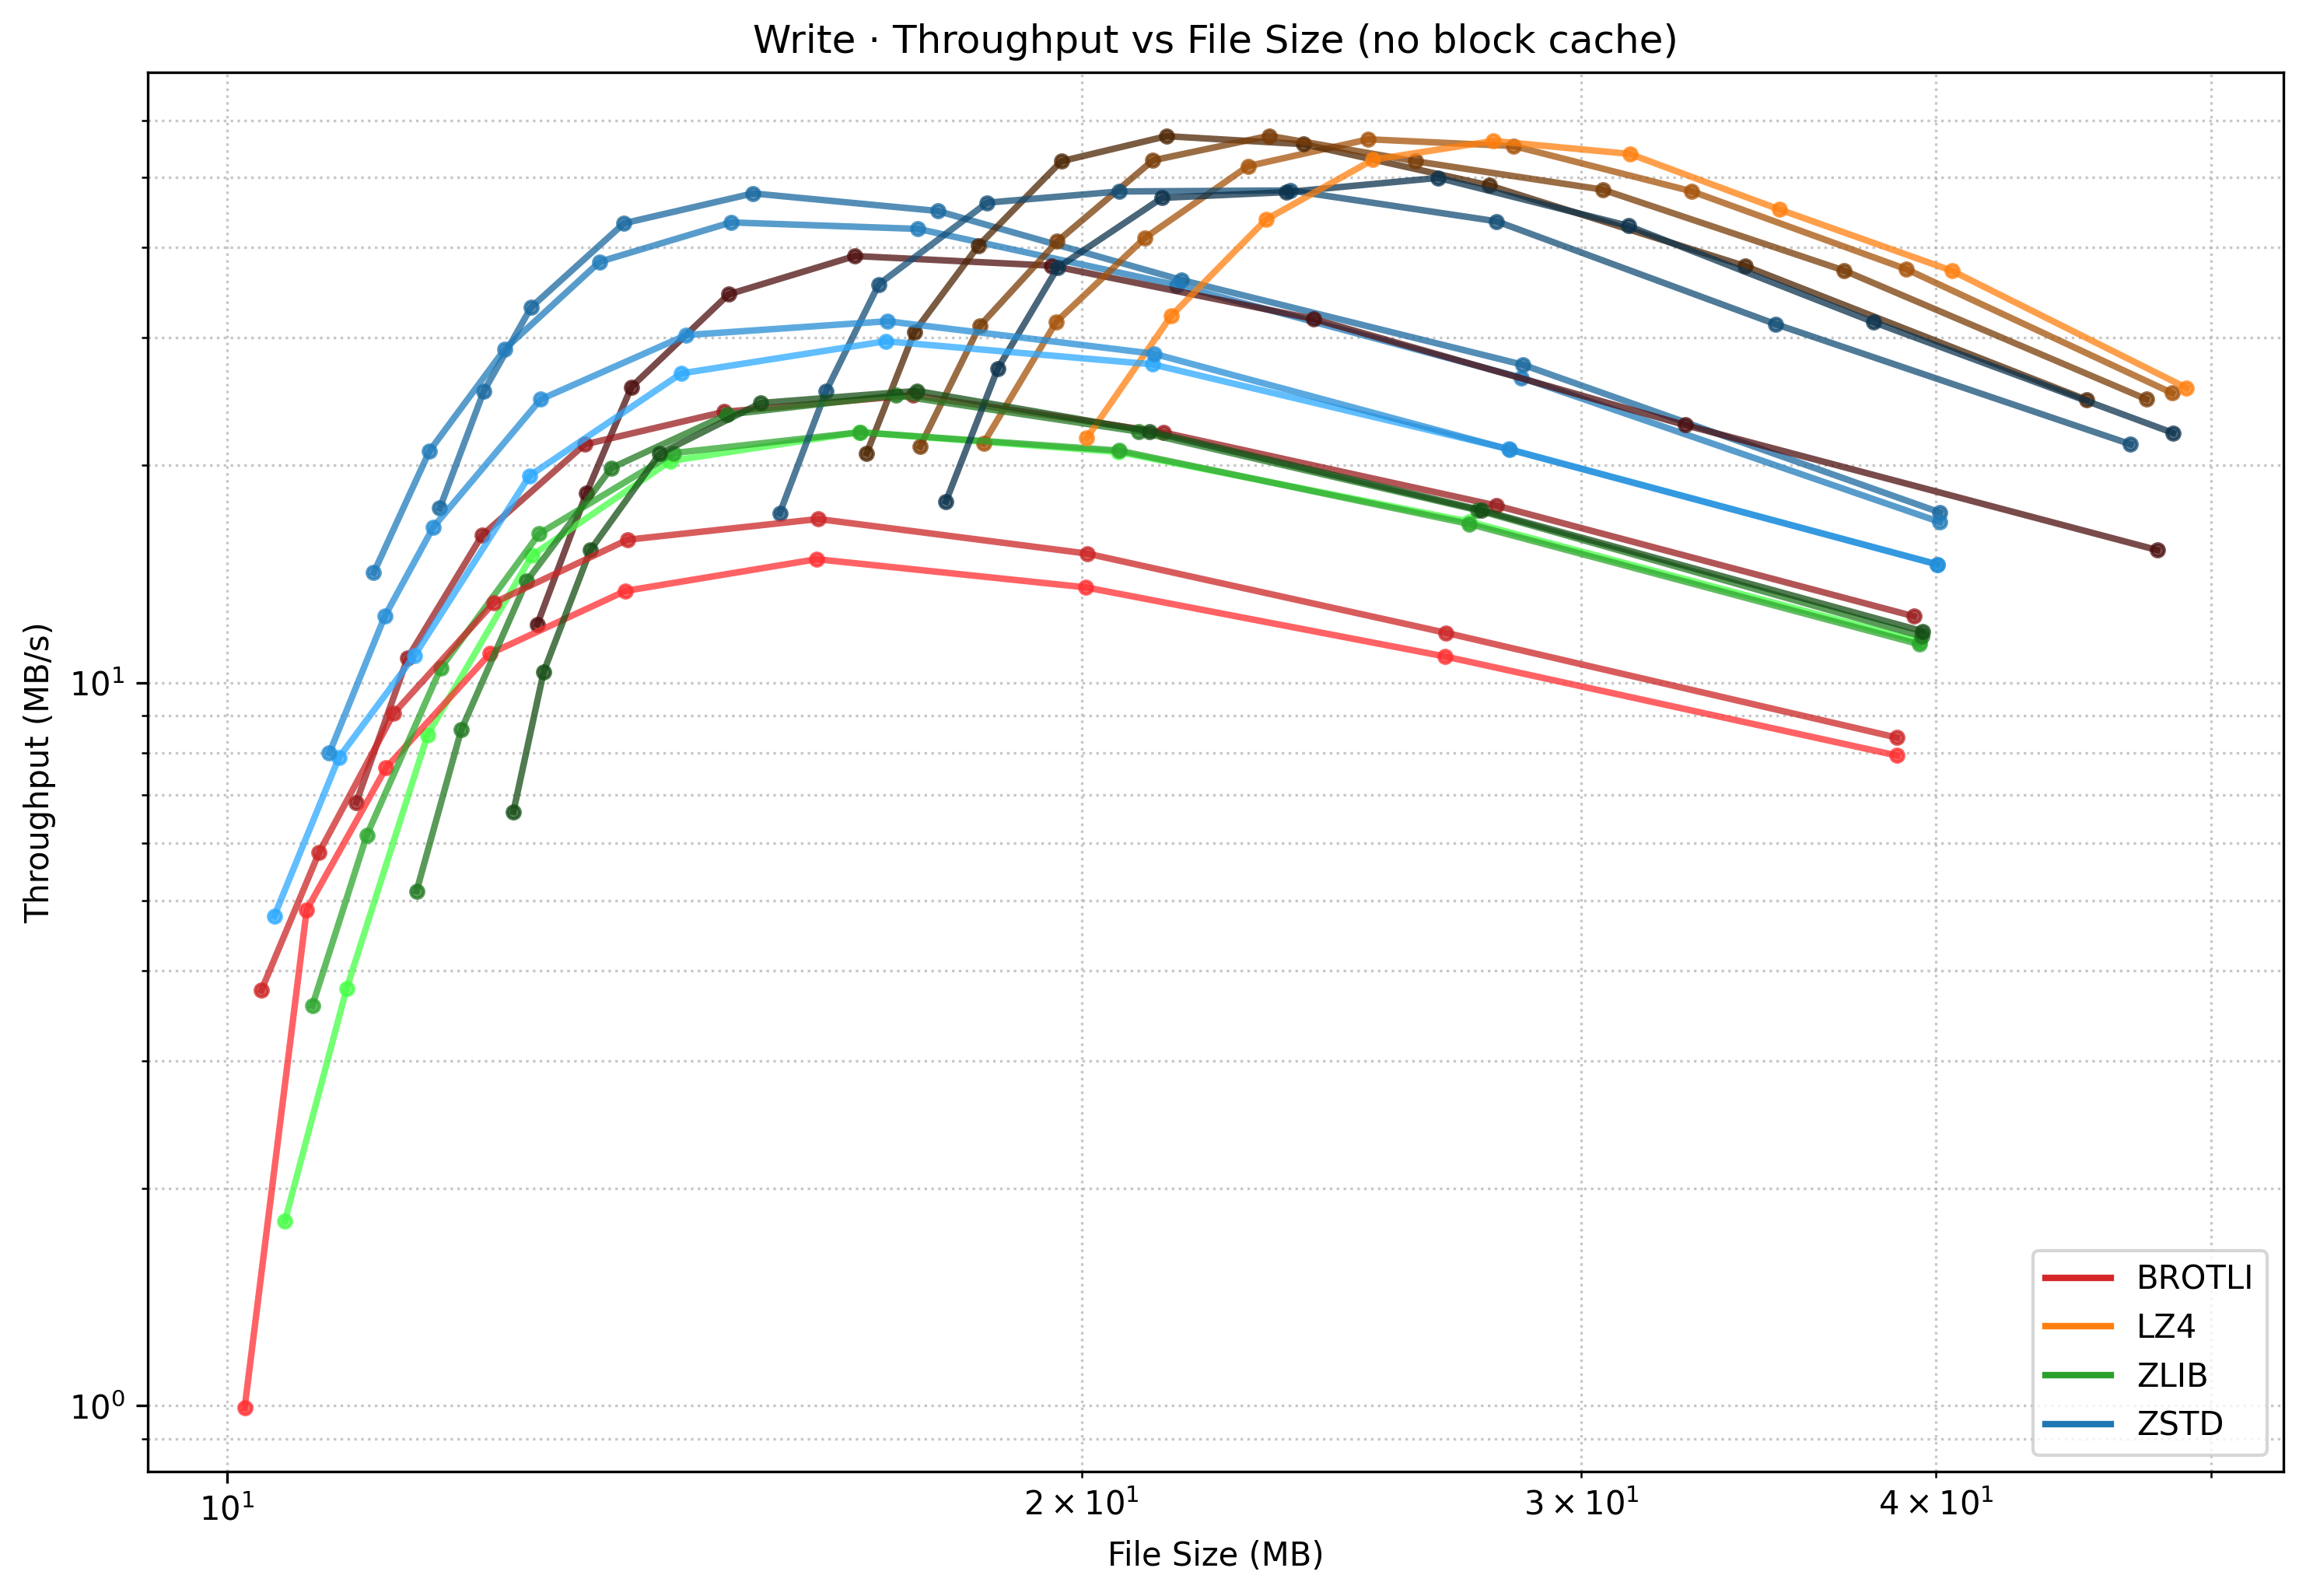
\includegraphics[width=\textwidth]{images/algorithms_no_cache.png}
    \caption{Сравнение алгоритмов сжатия при различных размерах блока: влияние на скорость произвольной записи и размер архива. Кэш отключён.}
    \label{fig:algorithms_no_cache}
\end{figure}

Общая для всех алгоритмов тенденция такова: при переходе к очень большим блокам (левая часть графика) скорость записи значительно падает, тогда как размер файла уменьшается уже несущественно. При чрезмерно малых блоках (правая часть) размер архива резко возрастает, а скорость, достигнув максимума в районе 16--32 КБ, начинает снижаться.

Среди рассмотренных компрессоров наиболее сбалансированным оказывается Zstd с уровнем сжатия 1: в диапазоне \texttt{block\_size} 4--16 КБ его точки лежат вблизи Pareto-фронта, уступая по скорости только LZ4, но давая заметно меньший размер файла. LZ4 демонстрирует наивысшую скорость записи, однако ценой большего объёма архива. Brotli обеспечивает наилучшее сжатие, но заметно медленнее; Zlib проигрывает Zstd и по скорости, и по степени сжатия.

\paragraph{Вывод.}
Полученные данные позволяют рекомендовать диапазон размеров блока 4--16 КБ как оптимальный для сценариев произвольной записи. В качестве универсального компрессора, предлагающего наилучший компромисс между скоростью и сжатием, целесообразно использовать Zstd с уровнем сжатия 1.
\subsection{Анализ накладных расходов}

\paragraph{Структура размера архива.}
Общий размер файла-контейнера можно представить как сумму трёх компонент:
\begin{enumerate}
    \item Базовый объём сжатых данных, который получился бы при сжатии всего файла одним блоком (непрерывным потоком).
    \item Потери от блочного сжатия --- избыточность, вызванная независимым сжатием каждого блока (потеря общего контекста).
    \item Метаданные библиотеки --- B-дерево, заголовок, таблица файлов, служебные поля блоков.
\end{enumerate}

Для того чтобы оценить вклад каждой части, выполнен следующий замер. Для файла \texttt{webster} (32 МБ) и компрессора Zstd-1 строились архивы с разными \texttt{block\_size}. Вычислялся размер базового сжатого потока (100\%). Затем вычислялись, в процентах от этой базы, оверхед, вызванный блочным разбиением (красный), и оверхед метаданных (голубой). Суммарная высота столбца может превышать 100\%, что означает, что полный размер архива более чем вдвое превышает размер непрерывно сжатых данных.

\paragraph{Результаты.}
Рис.~\ref{fig:overhead} показывает распределение накладных расходов.

\begin{figure}[h]
    \centering
    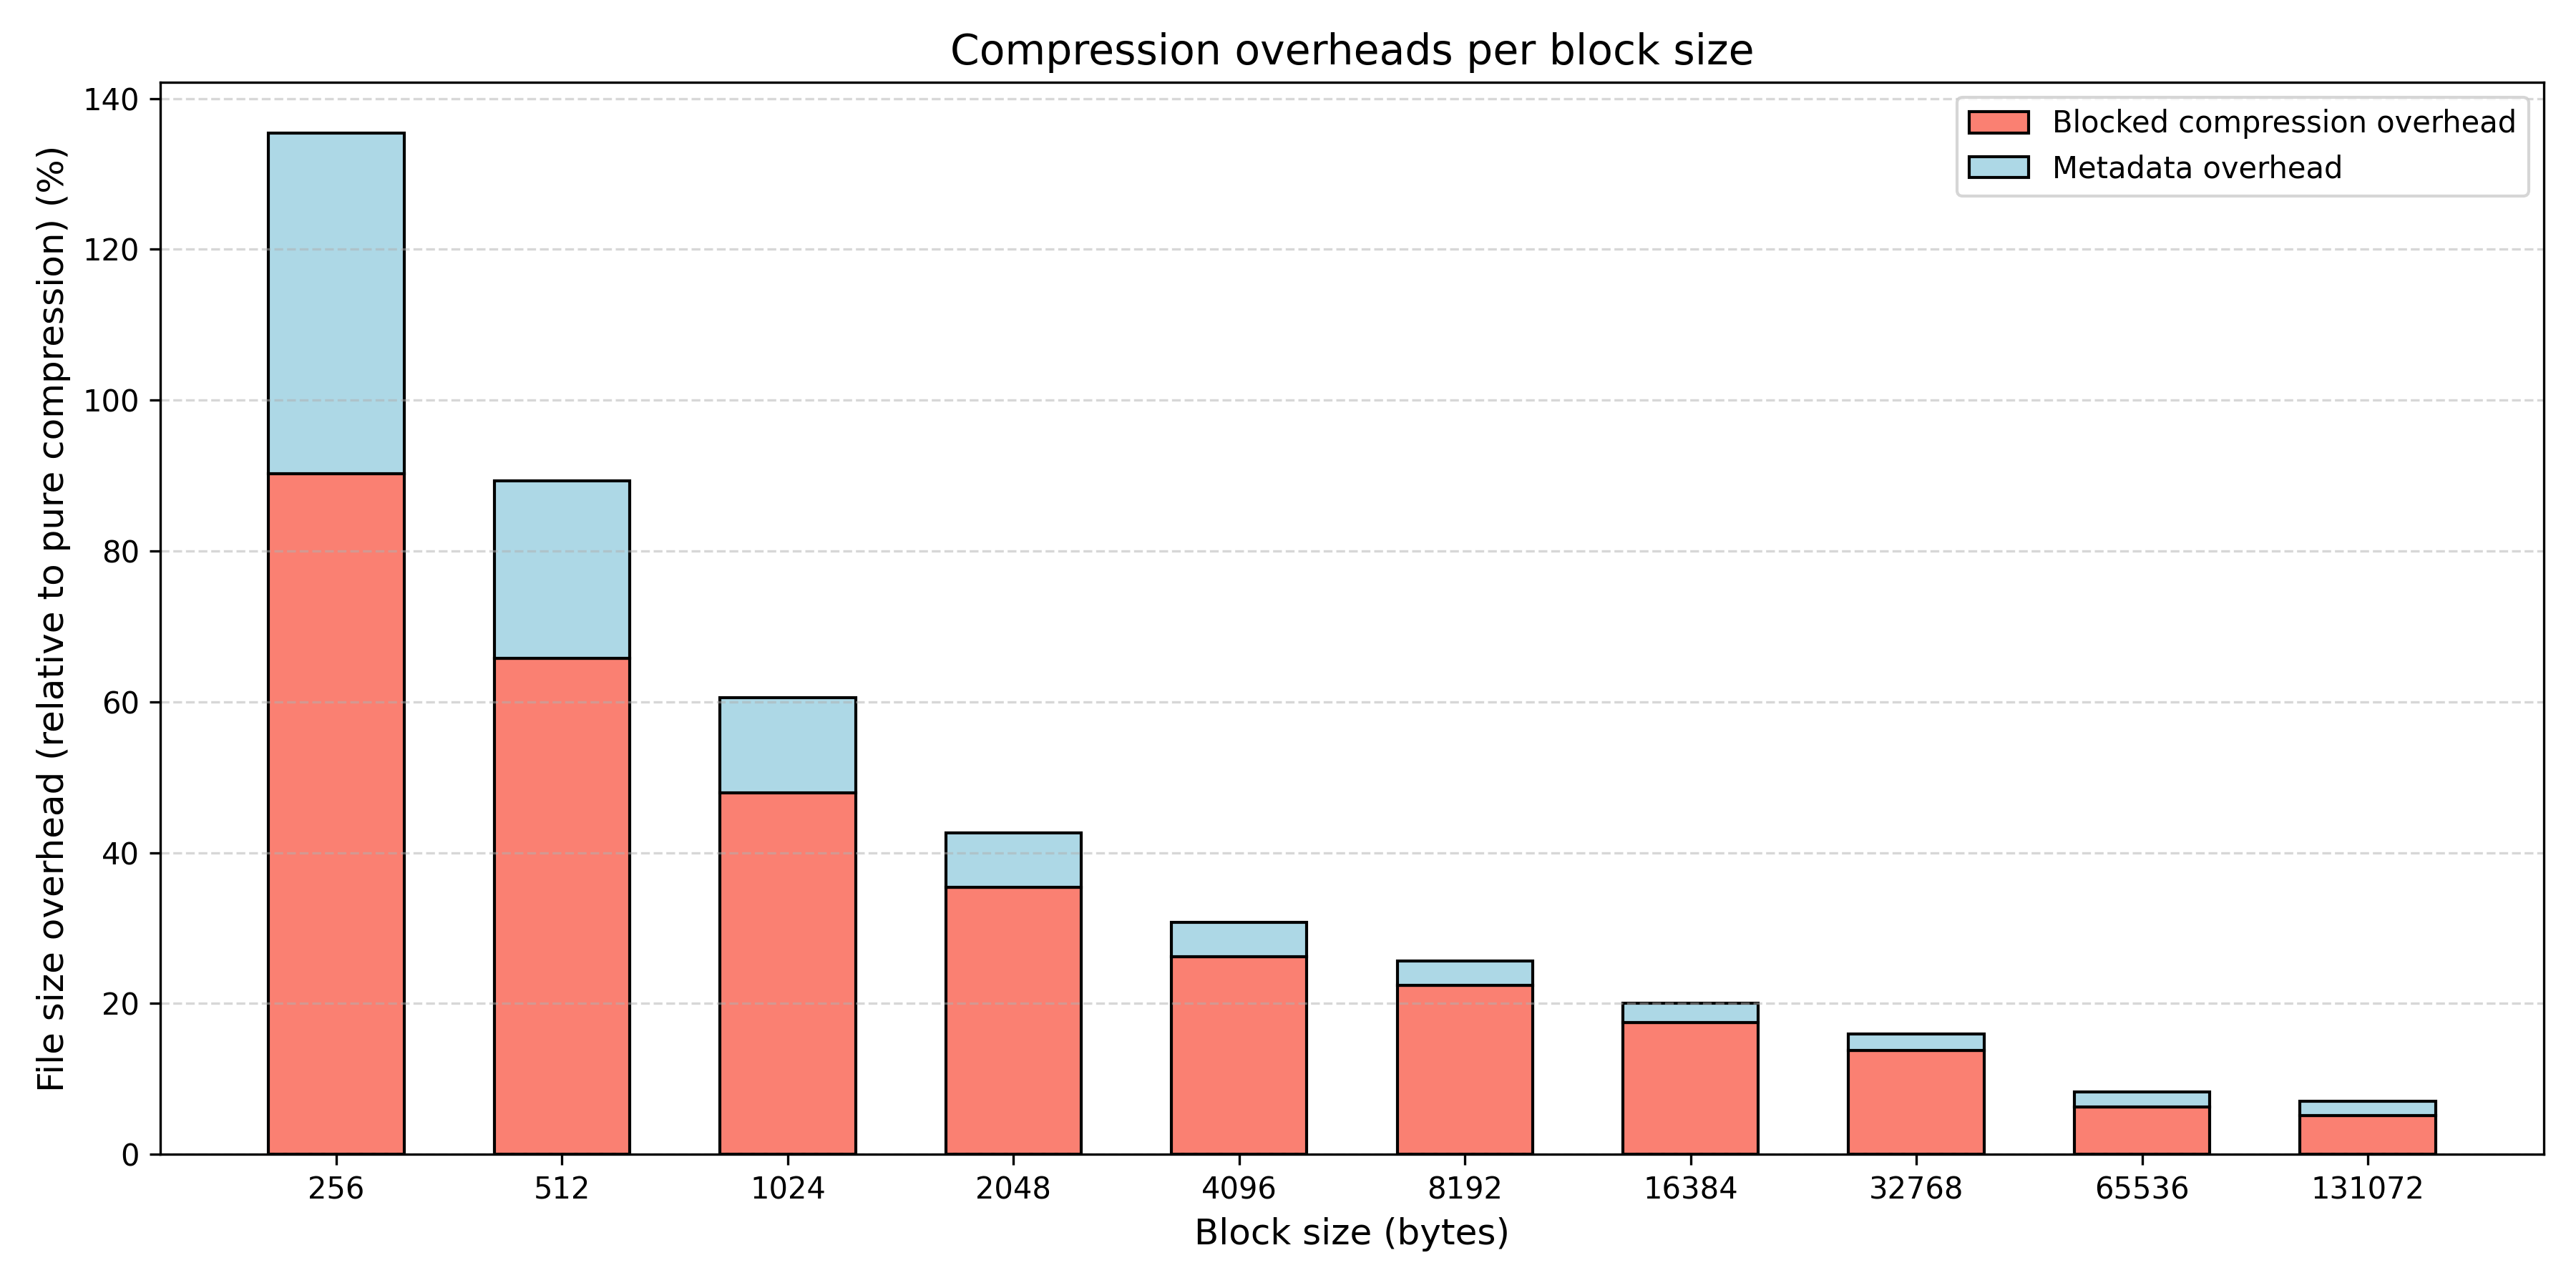
\includegraphics[width=\textwidth]{images/overhead_bars.png}
    \caption{Распределение накладных расходов в зависимости от размера блока (база~--- размер непрерывно сжатых данных).}
    \label{fig:overhead}
\end{figure}

При размере блока 8 КБ потери от блочного сжатия составляют около 25\%, а метаданные добавляют около 4\%. При увеличении блока потери от блочного сжатия убывают, стремясь к нулю, тогда как доля метаданных сокращается медленно и даже для крупных блоков остаётся на уровне нескольких процентов. При очень маленьких блоках (1 КБ) суммарный оверхед превышает 100\%, что делает такие размеры неприемлемыми.

\paragraph{Вывод.}
Собственные накладные расходы библиотеки (метаданные) невелики и не являются узким местом. Основной «платой» за произвольный доступ выступает ухудшение сжатия из-за независимой обработки блоков. Диапазон 4--16 КБ удерживает этот оверхед в разумных пределах (20--30\%), одновременно обеспечивая высокую скорость доступа, что согласуется с предыдущими рекомендациями.

\subsection{Итоги экспериментов}

Проведённые измерения подтверждают, что архитектурные решения, заложенные в Compio, работают на практике:

\begin{itemize}
    \item Механизм границ \texttt{block\_size\_min/max} успешно предотвращает неограниченное измельчение блоков и падение производительности при длительных сериях вставок и удалений.
    \item По скорости произвольного чтения Compio не уступает специализированным инструментам (seekable zstd, zran), предоставляя уникальную возможность модификации --- записи, вставки и удаления --- без полной перепаковки архива.
    \item Система кэширования делает библиотеку особенно эффективной при высокой локальности обращений, позволяя на чтении превосходить даже несжатый stdio, а на записи достигать сравнимых скоростей.
    \item Пользователь может гибко настраивать компромисс «скорость – степень сжатия», выбирая компрессор и размер блока. Рекомендованный диапазон размеров блока 4--16 КБ с компрессором Zstd-1 обеспечивает наилучший баланс.
    \item Накладные расходы библиотеки (метаданные) остаются скромными; основной источник увеличения размера архива --- потеря эффективности сжатия из-за блочной организации.
\end{itemize}